\documentclass[11pt]{article}
\pagestyle{empty}
\usepackage{color}
\usepackage{fancyhdr}
\usepackage{lastpage}
\pagestyle{fancy}
\renewcommand{\headrulewidth}{0pt}
\cfoot[R]{\thepage~of~\pageref{LastPage}}
\addtolength{\oddsidemargin}{-.875in}
\addtolength{\evensidemargin}{-.875in}
\addtolength{\textwidth}{1.75in}
\addtolength{\topmargin}{-.875in}
\addtolength{\textheight}{1.75in}
\usepackage{graphicx}
\graphicspath{ {/} }

\usepackage{amsfonts}
\usepackage{amsmath}
\usepackage{pgfplots}
\usepackage{minted}

\title{Cryptocurrencies and Decentralized Ledgers Homework 2}
\author{quentin.mcgaw (qm301)}
\date{October 2017}

\begin{document}

\maketitle

\begin{enumerate}

\item \textbf{\textcolor{blue}{Multi-judge escrow service: In class we saw how to use 2-out-of-3 multisig to build an escrow service where Alice can buy a product from Bob and, if all goes well, Alice gets the product and Bob gets paid. Otherwise a judge can adjudicate the dispute. One issue with that protocol is that the judge may demand a service fee and the participants, Alice and Bob, have no choice but to pay. In this question your goal is to design an escrow system where, ahead of time, Alice and Bob agree on the set of three judges so that during adjudication they can choose any one of the three to adjudicate. We are assuming that the three judges are honest and consistent, that is, all three will always rule the same way.}}
    \begin{enumerate}
    \item \textbf{\textcolor{blue}{Show how to implement a three-judge escrow system using a single standard multisig transaction to a multisig address that Alice and Bob agree on ahead of time. Your design must ensure that even if the three judges collude, they cannot steal the funds that Alice sends to Bob. Recall that if all goes well then the parties need not involve the judges. If
    something goes wrong, then any one of the three judges can adjudicate. Hint : You will need to use more than 5 keys in the multisig transaction. Alice and Bob will use more than one key each.}}
        \\ To achieve this, we need the following requirements:
        \begin{itemize}
            \item Alice's and Bob's signatures together \textbf{match} the threshold
            \item Alice's and any one of the judges' signatures together \textbf{match} the threshold
            \item Bob's and any one of the judges' signatures together \textbf{match} the threshold
            \item Alice's signature(s) \textbf{does not match} the threshold
            \item Bob's signature(s) \textbf{does not match} the threshold
            \item All the judge's signatures together \textbf{does not match} the threshold
        \end{itemize}
        \\ The solution to do this in a standard MULTISIG transaction with the least possible number of keys is to use 9 keys in the following agencement:
        \begin{itemize}
            \item 3 keys owned by Alice
            \item 3 keys owned by Bob
            \item 1 key owned by each judge
            \item The threshold set to 4
        \end{itemize}
        \\ The corresponding script is:
        \begin{minted}{python}
4 <pub_Alice1> <pub_Alice2> <pub_Alice3> <pub_Bob1> <pub_Bob2> <pub_Bob3> 
<pub_Judge1> <pub_Judge2> <pub_Judge3> 9 OP_CHECKMULTISIGVERIFY
        \end{minted}
    
    \item \textbf{\textcolor{blue}{Your solution from part (a) uses a standard multisig transaction, but the script must list more than five public keys. Write a script to achieve the same thing where each party is only assigned one key (only five keys total are listed in the redeem script) Hint : you'll need to use logical operations (e.g. $OP\_IF$, $OP\_OR$) in a non-standard script}}
        \\ We basically want the following logic implemented: 
        \\ (\textbf{BOB} AND \textbf{ALICE}) OR (\textbf{BOB} AND (\textbf{JUDGE1} OR \textbf{JUDGE2} OR \textbf{JUDGE3})) OR (\textbf{ALICE} AND (\textbf{JUDGE1} OR \textbf{JUDGE2} OR \textbf{JUDGE3}))
        \\ To adapt this logic to the script language, we ask the following questions and we have the following consequences:
        \newline
        \\ Did Bob sign?
        \begin{enumerate}
            \item YES: Did Alice sign?
            \begin{enumerate}
                \item YES: SUCCESS
                \item NO: Did any of the 3 judges sign?
                \begin{itemize}
                    \item YES: SUCCESS
                    \item NO: FAILURE
                \end{itemize}
            \end{enumerate}
            \item NO: Did Alice sign?
            \begin{enumerate}
                \item YES: Did any of the 3 judges sign?
                \begin{itemize}
                    \item YES: SUCCESS
                    \item NO: FAILURE
                \end{itemize}
                \item NO: FAILURE
            \end{enumerate}
        \end{enumerate}
        \newline
        \\ The following Bitcoin script hence matches the requirements:
        \begin{minted}{python}
<sig_bob> OP_0 <sig_judge2>
<pub_bob> OP_CHECKSIG
    OP_IF <pub_alice> OP_CHECKSIG
        OP_IF OP_VERIFY 
        OP_ELSE 1 <pub_judge1> <pub_judge2> <pub_judge3> 3 OP_CHECKMULTISIGVERIFY
        OP_ENDIF
    OP_ELSE <pub_alice> OP_CHECKSIGVERIFY 1 <pub_judge1> <pub_judge2> <pub_judge3> 
              3 OP_CHECKMULTISIGVERIFY
    OP_ENDIF
        \end{minted}
        \\ Note that the first line
        \begin{minted}{python}
        <sig_bob> OP_0 <sig_judge2>
        \end{minted}
        \\ is just an example, it could be all the possible combinations required, as long as they are placed in the right order (Bob, Alice first, then OP\_0 then judge(s))
        \\ In one line, the script looks like the following:
        \begin{minted}{python}
<sig_bob> OP_0 <sig_judge2> <pub_bob> OP_CHECKSIG OP_IF <pub_alice> OP_CHECKSIG 
OP_IF OP_VERIFY OP_ELSE 1 <pub_judge1> <pub_judge2> <pub_judge3> 3 
OP_CHECKMULTISIGVERIFY OP_ENDIF OP_ELSE <pub_alice> OP_CHECKSIGVERIFY 1 
<pub_judge1> <pub_judge2> <pub_judge3> 3 OP_CHECKMULTISIGVERIFY OP_ENDIF
        \end{minted}
        
        
    \end{enumerate}

\item \textbf{\textcolor{blue}{Network propagation: Assume a simple model for how quickly Bitcoin blocks propagate through the network: after $t$ seconds, a group of miners controlling a proportion $\alpha(t)$ of the mining power has heard about the transaction, up to some point $t_{max}$ after which all miners will have heard about it. That is, $\alpha(t) = 1$ for all $t \geq t_{max}$. Further assume that $\alpha(0) = 0$ and $\alpha(t)$ is monotonically increasing in $t$. Assume that blocks are found in Poisson process with a mean time to find a block of $\beta = 600$ seconds ($\lambda = 1/600$). A stale block (likely to become an orphan block) occurs if some miner finds a block before news of the most recent block reaches them.}}
    \begin{enumerate}
    \item \textbf{\textcolor{blue}{Given the design of the Bitcoin P2P network, explain why an exponential propagation model (i.e. $\alpha(t) \propto b^t$ for some $b$) is a plausible model.
    \\ Hint: Recall that the derivative of an exponential is another exponential function.}}
        \\ As block finding is a homogeneous Poisson process, the lengths of the inter-arrival times (which is the time to find the next block) follows the exponential distribution with mean $\frac{1}{\lambda} = 600$ seconds.
        \\ This is also plausible as the Bitcoin P2P network is an acyclic directed random graph, hence making propapagation through it exponential.
    
    \item \textbf{\textcolor{blue}{Suppose $\alpha(t) = 2^{t/30} - 1$, that is, an exponentially increasing proportion of the mining power hears about a new block up until $t_{max} = 30$ seconds, at which point all have heard. What is the probability of at least one stale block being found? 
    \\ Note: You do not need to solve the integral analytically. You may use a computer.}}
        \\ The probability to find at least one stale block is equal to the probability of finding at least 2 blocks in 600 seconds times the probability of the times at which any of the two blocks were found to be separated by less than 30 seconds. 
        \\ The probability of finding at least 2 blocks in 600 seconds is given by:
        \\ $P(k \geq 2) = \int_{2}^{\infty} \frac{\lambda^k e^{-\lambda}}{k!} dk = \int_{2}^{\infty} \frac{1^k e^{-1}}{k!} dk = \int_{2}^{\infty} \frac{e^{-1}}{k!} dk \approx 0.15802$
        \\ One (desperate) answer is that the probability of finding at least one stale block is equal to 1, because the question does not precise on which time range the stale block should be found. Because the probability of finding at least 2 blocks is 0.15802 and the probability that at least 2 or more blocks are found less than 30 seconds apart is also non-zero, the probability to find at least one stale block is 1 generally speaking.

    \item \textbf{\textcolor{blue}{If we lowered $\beta$ to 60 seconds to make transactions post faster, how would this affect your answer from part (b)? What problems might this cause?}}
        \\ In this case, 
        \\ The probability to find at least 2 blocks in $\beta = 60$ seconds is still 0.15802.
        \\ However, the probability that any of the 2 blocks found are separated by less than 30 seconds is much higher, if the same function $\alpha(t) = 2^{t/30} - 1$ is kept.
        \\ Therefore, with $\beta = 60$, the probability to find at least one stale block is much higher in this case.
        
    \item \textbf{\textcolor{blue}{One could argue that the increased rate of stale blocks identified in part (c) isn't really a problem as miners will still be paid at the same rate. Explain why this argument may not hold in practice. In particular, explain why the model for $\alpha(t)$ from part(b) is incomplete.}}
        \\ The network might start mining on top of the stale block or on top of the first block, depending on their localization. This would potentially lose time and power for half the network, and cause instability (i.e. 2 competing chains etc.). 
        \\ The model for $\alpha(t)$ is incomplete because it does not take into account the mining pools which would make $\alpha(t)$ not a perfect exponential but more of a "jumpy" function. 
    \end{enumerate}

\item \textbf{\textcolor{blue}{Power consumption: In this exercise we'll look at two ways to estimate the power consumption of the Bitcoin network. Assume in your answers that the difficulty of finding a bitcoin block is $d = 2^{72}$, the exchange rate is 1BTC= US \$4000 and that there are no transaction fees (only the fixed block reward of 12.5 BTC). Recall that energy is measured in joules (J) and power is in watts (W), where 1 W = 1 J/s.}}
    \begin{enumerate}
    \item \textbf{\textcolor{blue}{First, estimate the power consumption of the network assuming all mining rewards are spent on electricity. Assume all electricity is purchased at US industrial rates, which are about US\$0.05/kWH (and recall that 1 kWh = 3.6 MJ).}}
        \\ On average, the network gains $12.5 \text{ BTC/10 minutes} = 75 \text{ BTC/hour} = \text{US } \$ 300,000 \text{/hour}$.
        \\ In this case, on average, $\text{US } \$ 300,000 \text{/hour}$ would be spent on electricity, hence with a power consumption of $\frac{\text{US } \$ 300,000 \text{/hour}}{\text{US} \$ 0.05 \text{/kWH}} = 6,000,000 \text{ kW} = 6,000,000,000 \text{ W}$ overall.
    
    \item \textbf{\textcolor{blue}{Why might your estimate in part (a) be too high? Why might it be too low?}}
        \begin{itemize}
            \item It might be too high if the total network hash rate decreases until the next difficulty adjustment.
            \item It might be too low if the total network hash rate increases until the next difficulty adjustment.
        \end{itemize}
        
    \item \textbf{\textcolor{blue}{Next, estimate the power consumption of the entire network assuming all mining is being done with recent 16nm scale ASICs. Assume these devices can perform about $2^{33}$ SHA-256$^2$ computations per 1 J of electricity (about 0.1 J per GH).}}
        \begin{enumerate}
            \item With a difficulty $d = 2^{72}$, the network has to perform $d \times 2^{32} = 2^{104}$ SHA-256$^2$ operations in average to find a block.
            \item Because the difficulty adapts to the hash rate every 2016 blocks $\approx$ 2 weeks, we can say that the network has to perform $2^{104} \text{ SHA-256}^2 \text{ / 10 minutes}$ to find a block every 10 minutes on average.
            \item $2^{104}$ SHA-256$^2$ operations require $2^{104} \times \frac{1}{2^{33}} \text{ J} = 2^{71} \text{ J}$
            \item The network has thus a power consumption of $\frac{2^{71}}{600} \text{ W} = \frac{2^{68}}{75} \text{ W} \approx 3,935,305,402,391,371 \text{ kW}$
        \end{enumerate}
        
    \item \textbf{\textcolor{blue}{Why might your estimate in part (c) be too low? Why might it be too high?}}
        \begin{itemize}
            \item It might be too high if the total network hash rate decreases until the next difficulty adjustment.
            \item It might be too low if the total network hash rate increases until the next difficulty adjustment.
        \end{itemize}
    \end{enumerate}

\item \textbf{\textcolor{blue}{Post-block reward mining: Bitcoin's rules call for for fixed coinbase block rewards to disappear over time and be replaced by transaction fees as the sole source of revenue for miners. In this question we'll explore the implications of this transition on miner behavior.
\begin{itemize}
    \item Assume that the block size is increased so that miners can always include all available transactions in a block (e.g. assume blocks are essentially infinite).
    \item Assume that new transactions are broadcast at a constant rate, all including the same transaction fee. This means that the value of any block is directly proportional to the time since the last block was found. We'll say that the block reward is $R(t) = rt$ where $t$ is the time since the last block, and $r$ is a constant.
    \item Assume that all miners have the same cost to compute block hashes (e.g. to pay for the electricity for their mining hardware). We'll say the marginal cost of performing $d$ hashes is $c$, where $d$ is the current block difficulty (e.g. $d \cong 2^{72}$). We'll also assume that miners can turn their equipment on and off instantaneously and pay nothing when it's off.
\end{itemize}
Given these assumptions, miners clearly will not want to mine immediately after a block is found, as the value starts at 0, because the transaction pool is empty.}}
    \begin{enumerate}
    \item \textbf{\textcolor{blue}{How long will miners wait after a block is found before turning on their hardware?}}
        \begin{enumerate}
            \item Miners want to at least reach break-even on average with their revenues and losses.
            \item It takes $d \times 2^{32}$ SHA-256$^2$ in average to find a block.
            \item Miners will therefore wait for an average duration $t$ such that $R(t) = c \times 2^{32}$, before turning their hardware on.
        \end{enumerate}
    
    \item \textbf{\textcolor{blue}{Assume that the initial difficulty level $d_0$ is set to ensure the average block time would be $b=10$ minutes if all miners were mining constantly. After 2016 blocks using the above strategy, what will the new difficulty $d_1$ be (in terms of $b$, $c$, and $r$)? Assume the total amount of mining hardware is not changing.}}
        \begin{itemize}
            \item With the above strategy, miners wait for a duration $t_{wait} = \frac{c \times 2^{32}}{r}$ after a block is found.
            \item Miners would then have to spend $b$ minutes in average to find a block.
            \item The next difficulty $d_1$ would thus be less than $d_0$ to bring the average block finding time back from $b+t_{wait}$ to $b$ minutes. Therefore, $d_1 = d_0 \times \frac{b}{b+t_{wait}} = d_0 \times \frac{b}{b + \frac{c \times 2^{32}}{r}} = d_0 \times \frac{rb}{rb + c \times 2^{32}}$
        \end{itemize}
        
    \item \textbf{\textcolor{blue}{Will $d_2$ change again in the next round (assuming all of the parameters stay the same) or will it stay the same as $d_1$?}}
        \\ Now $c_1$ is the cost of performing $d_1$ hashes, which is reduced from the previous $c$ and we have $c_1 = c \times \frac{rb}{rb + c \times 2^{32}}$ (as we assumed $c$ to be proportional to $d$)
        \\ Therefore miners will now wait a reduced time $t_{wait1} = \frac{c \times \frac{rb}{rb + c \times 2^{32}} \times 2^{32}}{r} = \frac{c_1 \times 2^{32}}{r}$
        \\ $d_2$ will thus change again as miners are still waiting during $t_{wait1}$ before turning their hardware on, hence making the average time to find a block equal to $b + t_{wait1}$.
        
    \item \textbf{\textcolor{blue}{Another possible mining strategy is the following: immediately after a block is found, it is not profitable to attempt to find a new block (as the transaction pool is empty) but it is profitable to try to re-mine the previous block, mining $\epsilon$ fewer transactions so that mining on top of this new block will be more attractive than mining on top of the original block. Suppose you are the only miner executing this strategy. Suppose the previous block was found after $t_0$ time (so that the block reward for the previous is $rt_0$), and $t_1$ is the time since the previous block was found. For what value of $t_1$ should you switch from trying to steal the previous block, to trying to mine a fresh block?}}
        \begin{itemize}
            \item All the other miners turn their mining equipment on after a certain time $t_{wait}$ so that the pool of transactions contains enough fees to pay for the costs of mining.
            \item The block you would find would have an associated waiting time $t_{waitnew} = t_{wait} - t_{\epsilon}$ , where $t_{\epsilon}$ is the waiting time you offer to other miners by not including the $\epsilon$ transactions in your block.
            \item You must find a block such that $t_{waitnew} < t_{wait} - t_1$ in order to have other miners mine on top of your block.
            \item Therefore we have $t_{wait} - t_{\epsilon} < t_{wait} - t_1 \Rightarrow t_1 < t_{\epsilon}$. You should therefore stop at $t_1 = t_{\epsilon} - 1$. 
        \end{itemize}
    \end{enumerate}

\item \textbf{\textcolor{blue}{Feather forking: In class we learned about feather forking: a coalition of miners controlling a fraction $\alpha$ of the total mining power attempts to censor transactions by announcing: "if we see a block containing a transaction from our blacklist $B$, we will attempt to fork until we are 3 blocks behind the main chain." This strategy can be shown in a probabilistic state machine:}}
    \newline
    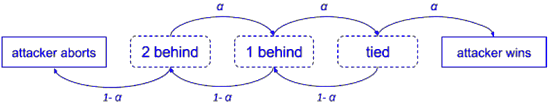
\includegraphics{diagram0.png}
    \begin{enumerate}
    \item \textbf{\textcolor{blue}{What is the probability that the censorship attack will succeed in terms of $\alpha$?
    \\ Hint: Express the probability of the fork succeeding from each active state in the state machine above as $p_0$, $p_1$ and $p_2$. You can now express each probability in terms of the others and solve a system of three equations for $p_1$, the probability of the attack succeeding from the start state, in terms of $\alpha$.}}
        \begin{itemize}
            \item When the situation is tied, the success probability is $p_0 = \alpha$
            \item When the attacker is 1 block behind, the success probability is $p_1 = \alpha p_0 + (1-\alpha)p_2$
            \item When the situation is 2 blocks behind, the success probability is $p_2 = \alpha p_1$
        \end{itemize}
        We want to find $p_1$ in terms of $\alpha$. We have:
        \\ $p_1 = \alpha p_0 + (1-\alpha)p_2$
        \\ $\Rightarrow p_1 = \alpha^2 + (1-\alpha)(\alpha p_1)$
        \\ $\Rightarrow p_1 = \alpha^2 + \alpha p_1 - \alpha^2 p_1$
        \\ $\Rightarrow p_1(\alpha^2 - \alpha + 1) = \alpha^2$
        \\ $\Rightarrow p_1 = \frac{\alpha^2}{\alpha^2 - \alpha + 1}$
        \\ Therefore the probability that the censorship attack will succeed is given by $p_1 = \frac{\alpha^2}{\alpha^2 - \alpha + 1}$.
        \newline
        \newline
        \begin{tikzpicture}
        \begin{axis}[
            axis lines = left,
            xlabel = $\alpha$,
            ylabel = {Probability},
        ]
        \addplot [
            domain=0:1, 
            samples=30, 
            color=red,
            ]
            {(x*x)/((x*x)-x+1)};
        \addlegendentry{$p_1 = \frac{\alpha^2}{\alpha^2 - \alpha + 1}$}
        \end{axis}
        \end{tikzpicture}
        \newline
        As expected, as $\alpha$ grows, $p_1$ grows almost proportionally.
    
    \item \textbf{\textcolor{blue}{On expectation, for how long (expressed as a number of blocks found) will the system be in a forked state after the attack is launched before it either succeeds or fails?
    \\ Hint: You can solve this problem using a similar system of equations as above, noting that every time a transition is taken the fork lasts one additional block. Make sure that, as a sanity check, the attack is expected to resolve in 2 blocks for both $\alpha \rightarrow 0$ and $\alpha \rightarrow 1$.}}
        \begin{itemize}
            \item When the situation is tied, there are $b_0 = (1 - \alpha)b_1 + 1$ additional blocks in average.
            \item When the attacker is 1 block behind, there are $b_1 = \alpha b_0 + (1 - \alpha)b_2 + 1$ additional blocks in average.
            \item When the situation is 2 blocks behind, there are $b_2 = \alpha b_1 + 1$ additional blocks in average.
        \end{itemize}
        We want to find $b_1$ in terms of $\alpha$:
        \\ $b_1 = \alpha b_0 + (1 - \alpha)b_2 + 1$
        \\ $\Rightarrow b_1 = \alpha ((1 - \alpha)b_1 + 1) + (1 - \alpha)(\alpha b_1 + 1) + 1$
        \\ $\Rightarrow b_1 = \alpha (b_1 - \alpha b_1 + 1) + \alpha b_1 + 1 - \alpha^2 b_1 - \alpha + 1$
        \\ $\Rightarrow b_1 = \alpha b_1 - \alpha^2 b_1 + \alpha + \alpha b_1 + 1 - \alpha^2 b_1 - \alpha + 1$
        \\ $\Rightarrow b_1 = -2 \alpha^2 b_1 + 2 \alpha b_1 + 2$
        \\ $\Rightarrow b_1(2 \alpha^2 - 2 \alpha + 1) = 2$
        \\ $\Rightarrow b_1 = \frac{2}{2 \alpha^2 - 2 \alpha + 1}$
        \\\\ The system will thus be in a forked state for $\frac{2}{2 \alpha^2 - 2 \alpha + 1}$ blocks on expectation.
        \newline
        \newline
        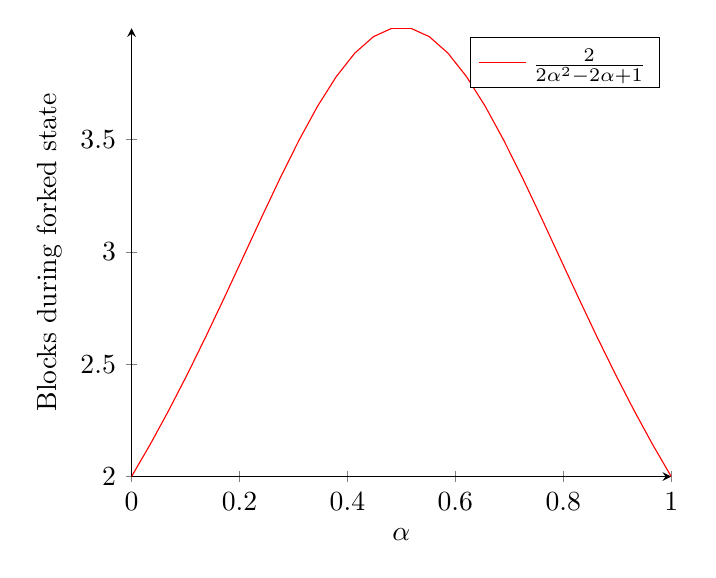
\begin{tikzpicture}
        \begin{axis}[
            axis lines = left,
            xlabel = $\alpha$,
            ylabel = {Blocks during forked state},
        ]
        \addplot [
            domain=0:1, 
            samples=30, 
            color=red,
            ]
            {2/(2*(x*x)-2*x+1)};
        \addlegendentry{$\frac{2}{2 \alpha^2 - 2 \alpha + 1}$}
        \end{axis}
        \end{tikzpicture}
        \newline
        As you can see on this graph, it's interesting to see that the peak of blocks would be reached when $\alpha = 0.5$, and is symmetric.
    \end{enumerate}

\item \textbf{\textcolor{blue}{Mining pool sabotage: Recall that mining pools enable individual miners to share risk and reward, lowering the variance of their earnings while keeping the same expected value. Participants repeatedly submit shares (blocks that are valid at a lower difficulty) to prove how much work they are doing. Whenever the pool finds a block, the coinbase from that block is split among the participants in proportion to the number of shares submitted. One risk is sabotage, in which a participant submits shares, but withholds full solutions if they are found.}}

    \begin{enumerate}
    \item \textbf{\textcolor{blue}{Consider two pools, $P_1$ and $P_2$ with mining power $\alpha_1$ and $\alpha_2$, respectively. What will $P_1$'s expected share of the total earnings be if it dedicates $\beta < \alpha_1$ power towards sabotaging $P_2$? Note that when $P_1$ finds a block it gets the entire coinbase. When $P_2$ finds a block, $P_1$ receives a fraction of the coinbase proportional to the number of shares $P_1$ generated while mining for $P_2$.
    \\ Hint: $P_2$'s total mining power is now $\alpha_2 + \beta$, but only $\alpha_2$ is used for finding a new block. Because $\beta$ power is no longer used to find blocks, $P_2$'s useful mining power, as a fraction of the entire network, is now $\alpha_2 / (1 - \beta)$. The same reasoning also applies to $P_1$. You may assume that the block discovery rate is always 10 minutes.}}
        \begin{itemize}
            \item The total mining power is now reduced from $1$ to $1 - \beta$
            \item $P_2$ gets $\frac{\alpha_2}{1 - \beta}$ share of the earnings from its own mining power and loses $\frac{\alpha_2}{1 - \beta} \times \frac{\beta}{\alpha_2 + \beta}$ share of the earnings to P1. Overall it earns $\frac{\alpha_2^2}{(1 - \beta)(\alpha_2 + \beta)}$  share of the earnings.
            \item $P_1$ gets $\frac{\alpha_1 - \beta}{1 - \beta}$ share of the earnings from its own mining power, plus $\frac{\alpha_2}{1 - \beta} \times \frac{\beta}{\alpha_2 + \beta}$  share of the earnings from the shares sent to $P_2$. Overall, $P_1$ receives $\frac{\alpha_1 - \beta}{1 - \beta} + \frac{\alpha_2 \beta}{(1 - \beta)(\alpha_2 + \beta)} = \frac{(\alpha_1 - \beta)(\alpha_2 + \beta) + \alpha_2 \beta}{(1 - \beta)(\alpha_2 + \beta)} = \frac{\alpha_1 \alpha_2 + \alpha_1 \beta - \alpha_2 \beta - \beta^2 + \alpha_2 \beta}{\alpha_2 + \beta - \alpha_2 \beta - \beta^2} = \frac{ - \beta^2  + \alpha_1 \beta + \alpha_1 \alpha_2}{- \beta^2 - \alpha_2 \beta + \beta + \alpha_2}$  share of the earnings.
        \end{itemize}
    
    \item \textbf{\textcolor{blue}{Provide concrete values for $\alpha_1$, $\alpha_2$, $\beta$ in which this attack is advantageous for $P_1$.}}
        \begin{itemize}
            \item $\alpha_1 = 0.4$
            \item $\alpha_2 = 0.3$
            \item $\beta = 0.08$
        \end{itemize}
        In this case, $P_1$ earns $0.41647597254004576$ share of earnings, which is above its $0.4$ normal share of earnings
        
    \item \textbf{\textcolor{blue}{Suppose $P_2$ wants to protect itself by kicking out participants observed to be reporting a suspiciously low rate of valid blocks compared to how many shares they report. Explain why this might inadvertently punish honest participants.}}
        \\ As finding a block is random, this might punish honest participants that actually find shares but not the block for a while. 
        \\ On the other hand, the longer $P_2$ waits without receiving a block from a miner, the most likely this miner is dishonest, although this could still be due to bad luck.
        
    \item \textbf{\textcolor{blue}{Suppose two pools, each with power $\alpha$, sabotage each other with power $\beta < \alpha$. For what range of $\beta$ will the two pools lose revenue by attacking each other? How much will they lose? What classic game from game theory is this situation an instance of?}}
        \begin{itemize}
            \item If there are other miners apart from these two pools, then they will both lose money for any $\beta > 0$. This is due to the fact that $2 \times \beta$ is removed from the network, so other miners will profit from $P_1$ AND $P_2$, but $P_1$ and $P_2$ will both lose $\beta$ share of earnings.
            \item If the only mining pools are $P_1$ and $P_2$, then they would have the same share of the earnings but would lose money until the difficulty adapts to their mutual sabotage, so to the overall useful mining power which is $2 \alpha - 2 \beta$.
        \end{itemize}
    \end{enumerate}
\end{enumerate}

\end{document}